\documentclass[a4paper,11pt]{article} % fonte 11 points, papier a4

\usepackage[english]{babel} % language options
%\usepackage{textcomp}

\usepackage[utf8]{inputenc}   % character coding
\usepackage{amsmath}	% utilisation de gather
\usepackage{amssymb}    % sets symbols
\usepackage{siunitx}  % degree symbol and other units
\usepackage{numprint} % number formatting
\npdecimalsign{.}

%\usepackage[top=2.5cm, bottom=2.5cm, left=3.0cm, right=3.0cm]{geometry} % page geometry
\usepackage[top=1.0in, bottom=1.0in, left=1in, right=1in]{geometry} % page geometry

\usepackage{graphicx}   % introduction de graphiques
\usepackage{float}
\graphicspath{{images/}{.}}
\DeclareGraphicsExtensions{.pdf, .eps,.png,.jpg}
\usepackage{subcaption}
\usepackage{epstopdf} % image eps
%\usepackage[font=scriptsize]{caption}
\usepackage[font=small]{caption}
\setlength{\belowcaptionskip}{-10pt}
\setlength{\abovecaptionskip}{5pt}
%\usepackage{pdfpages} 	% Permet d'inclure des pages pdf.
%\usepackage{amssymb} % R symbol : $\mathbb{R}$

%\usepackage{listings}
%\usepackage{enumerate}



\usepackage{fancyhdr}	% en tete de page
\renewcommand{\headrulewidth}{0pt}
\setlength{\headheight}{15pt}
\fancypagestyle{plain}{%
  \fancyhf{}% Clear header/footer
  \fancyhead[L]{\color{gray}Ruslan Aydarkhanov and Florian Borse}% Right header
  \fancyfoot[C]{\color{gray}\thepage}% Right header
}
\pagestyle{plain}
%\pagestyle{empty}
%\pagestyle{headings}
%\addtolength{\textwidth}{1cm} %modifier les marges
%\addtolength{\hoffset}{-1cm}
%\addtolength{\textwidth}{2cm} 

% Sections
\usepackage{titlesec}
\titleformat{\section}{\large\bfseries}{Exercise \thesection.}{.35em}{}
%\renewcommand\thesubsection{(\alph{subsection})}
\titleformat{\subsection}{\itshape}{\thesubsection}{.35em}{}

% Hyper
%\usepackage[table,usenames,dvipsnames]{xcolor}
%\usepackage{hyperref} % Required for adding links   and customizing them
%\definecolor{linkcolour}{rgb}{0,0.2,0.6} % Link color
%\hypersetup{colorlinks,breaklinks,urlcolor=linkcolour,linkcolor=linkcolour} % Set link colors throughout the document


%%%%
% TODO PACKAGE
% Commands:
% - \missingfigure{Make a sketch of the structure of a trebuchet.}
% - \todo[inline,color=blue!20]{Put different methods until now + papers method}%
%\usepackage[colorinlistoftodos,disable]{todonotes} % Disable TODO
\usepackage[colorinlistoftodos]{todonotes} % Enable TODO
\newcommand{\todob}[1]{\todo[color=blue!20]{#1}}
\newcommand{\todobl}[1]{\todo[inline,color=blue!20]{#1}}
%%%%

%\setcounter
%###################
%% Début du document
%###################
\begin{document}

\begin{center}
    \bfseries\Large
    MiniProject:\\
    Modeling pacemaker neurons\\
    with the Hodgkin-Huxley model

\end{center}
%##################
%##################
\section{Introduction}
To understand a complex neural network, one has to know not only how its
neurons are connected together, but also how each of them behave.
This has been the main concern of Hodgkin and Huxley when they created
their model to describe how a neuron behaves, under different circumstances
and in terms of ions, currents and voltages.

This model considers the electric behaviour of a neuron as flows of ions
through a membrane, either through channels or by a pump, the flows being
derived by the difference in potential. The classic way to represent the
behaviour of a membrane is therefore by setting that the difference in
potential is the sum of all flows :
\begin{align*}\frac{dV}{dt} = [I_{ext}+g_{Na}(E_{Na}-V)+g_K(E_K-V)+\frac{g_l}{C_m}(E_l-V)]\end{align*}

There are several interesting terms in this equation : $g_{Na}(E_{Na}-V)$
describes how the sodium current is influenced by the difference in
potential between the interior and the exterior of the neuron, $g_K(E_K-V)$
does the same with potassium. $\frac{g_l}{C_m}(E_l-V)$ describes the
leakage of the neuron, and $I_{ext}$ describes one of the values we want
to play with, which is the current we inject into the neuron so it can
actually have an interesting reaction, other than equilibrium.

One important concept is the gating variable. To emulate correctly how
a neuron behaves in terms of ion currents, we need to assess if their
specific channels are open or not. To model the behaviour of a channel,
one uses gating variables, which in our model are used as follow :
$g_K$ depends on $n^4$ and $g_{Na}$ on $m^3(1-n)$. This permits us to
define an effective conductance of a channel. The variables behave as
described by the set of equations (2) from the project description.

The goal of this project is of course not only to create an in silico
implementation of the Hodgkin-Huxley model using Brian, and playing with
it as such, but throughout the project we also create other classes of
channels, such that the neurons start undergoing other behaviours, to
emulate behaviours different classes of neurons actually have in vivo.

\section{HH simulation}

In this section, we test our implementation of the Hudgkin-Huxley model.
We inject a current of 100 pA into our neuron for 100 ms, as we see in
the second subplot. By looking at the first subplot, it becomes obvious
that the current raises the base potential of the neuron from a bit
more than -70 to a bit more than -50.

By looking at the third subplot, one can observe that this raise in
base potential affects the gating variables m and n : both react to
this change, but m reacts much quicker, which has an opening effect
on the sodium channel, since it is to the power of 3 whereas the closing
effect of n is to the power of 1 only.

As the sodium channels open more and more, the difference from the
base potential becomes bigger and bigger, which in turn increases the
gating variables more and more : the inflow of sodium increases more
and more, taking a spike-like shape.

But the difference from base potential also starts having a big effect
on n for the potassium channels, since there it is of power 4 : at
some point, the potassium channels open, and since the slope of the
induced current is very steep and negative to the sodium's, the already
steep increase of voltage becomes countered by a steeper decrease.
The potential stops increasing abruptly and decreases very quickly.
This accounts for the spikey behaviour of the potential during action
potential.

\begin{figure}[H]
    \centering
    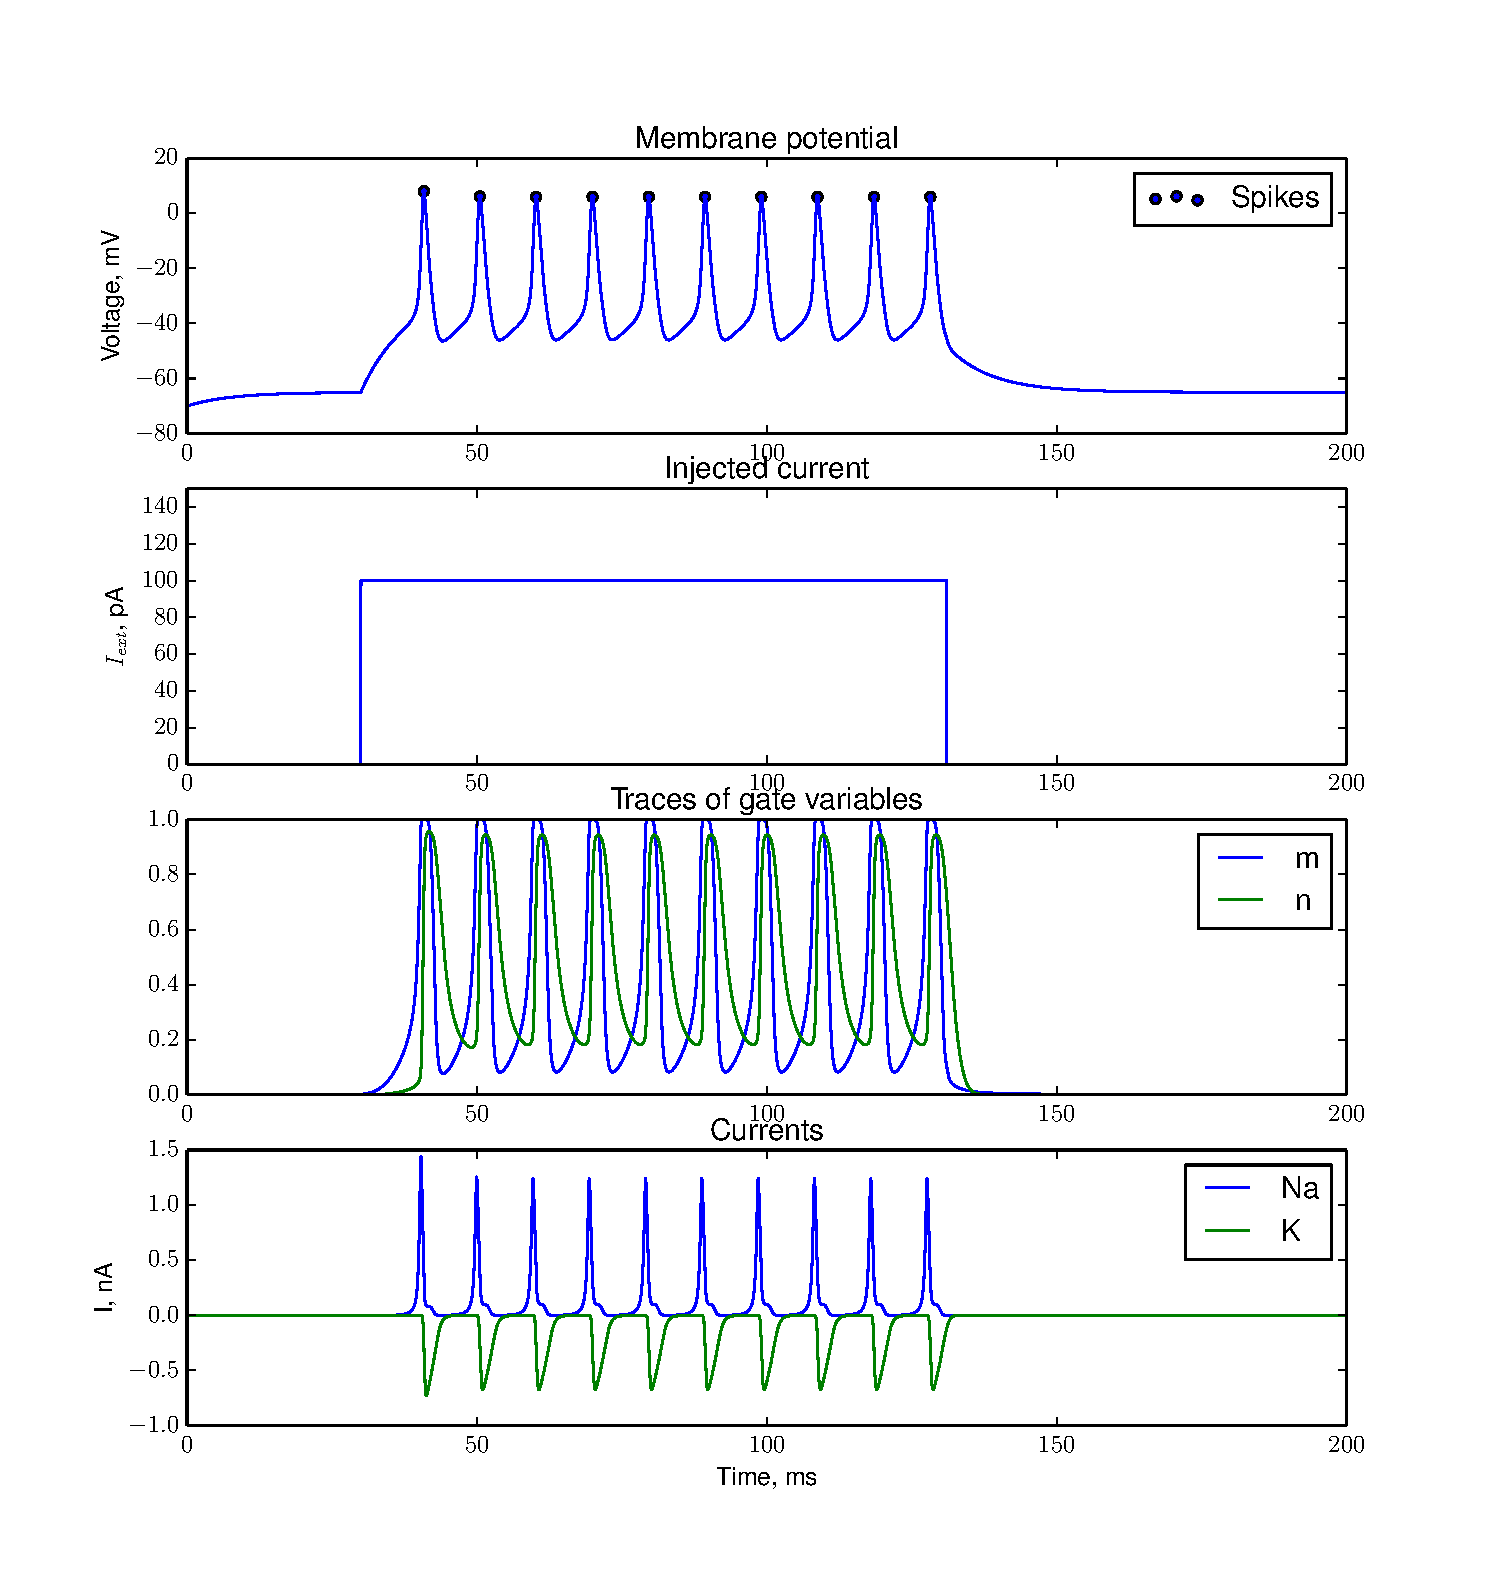
\includegraphics[width=\textwidth]{step_cur}
    \caption{Step current}
    \label{fig:step}
\end{figure}

This sudden decrease in potential has an effect on the gating variables
: they decrease abruptly too. Quickly, both inflow of sodium and
outflow of potassium decrease, which affects m quicker than n as
we see in the third subplot. This way, the potassium outflow can
still have an effect on m, but much slower. Finally, the sodium channel
closes again, followed by the potassium channel, and the voltage
is back to the input current induced potential.

Figure 2 gives a nice view of the difference in time constant,
the first subplot indicating to us how much this difference gets
at the voltages we consider. On the second figure, again, we can
see the difference of time constant, and how m reacts sooner than
n. What we also see, is that the increase in m is smaller than
that of n.

\begin{figure}[H]
    \centering
    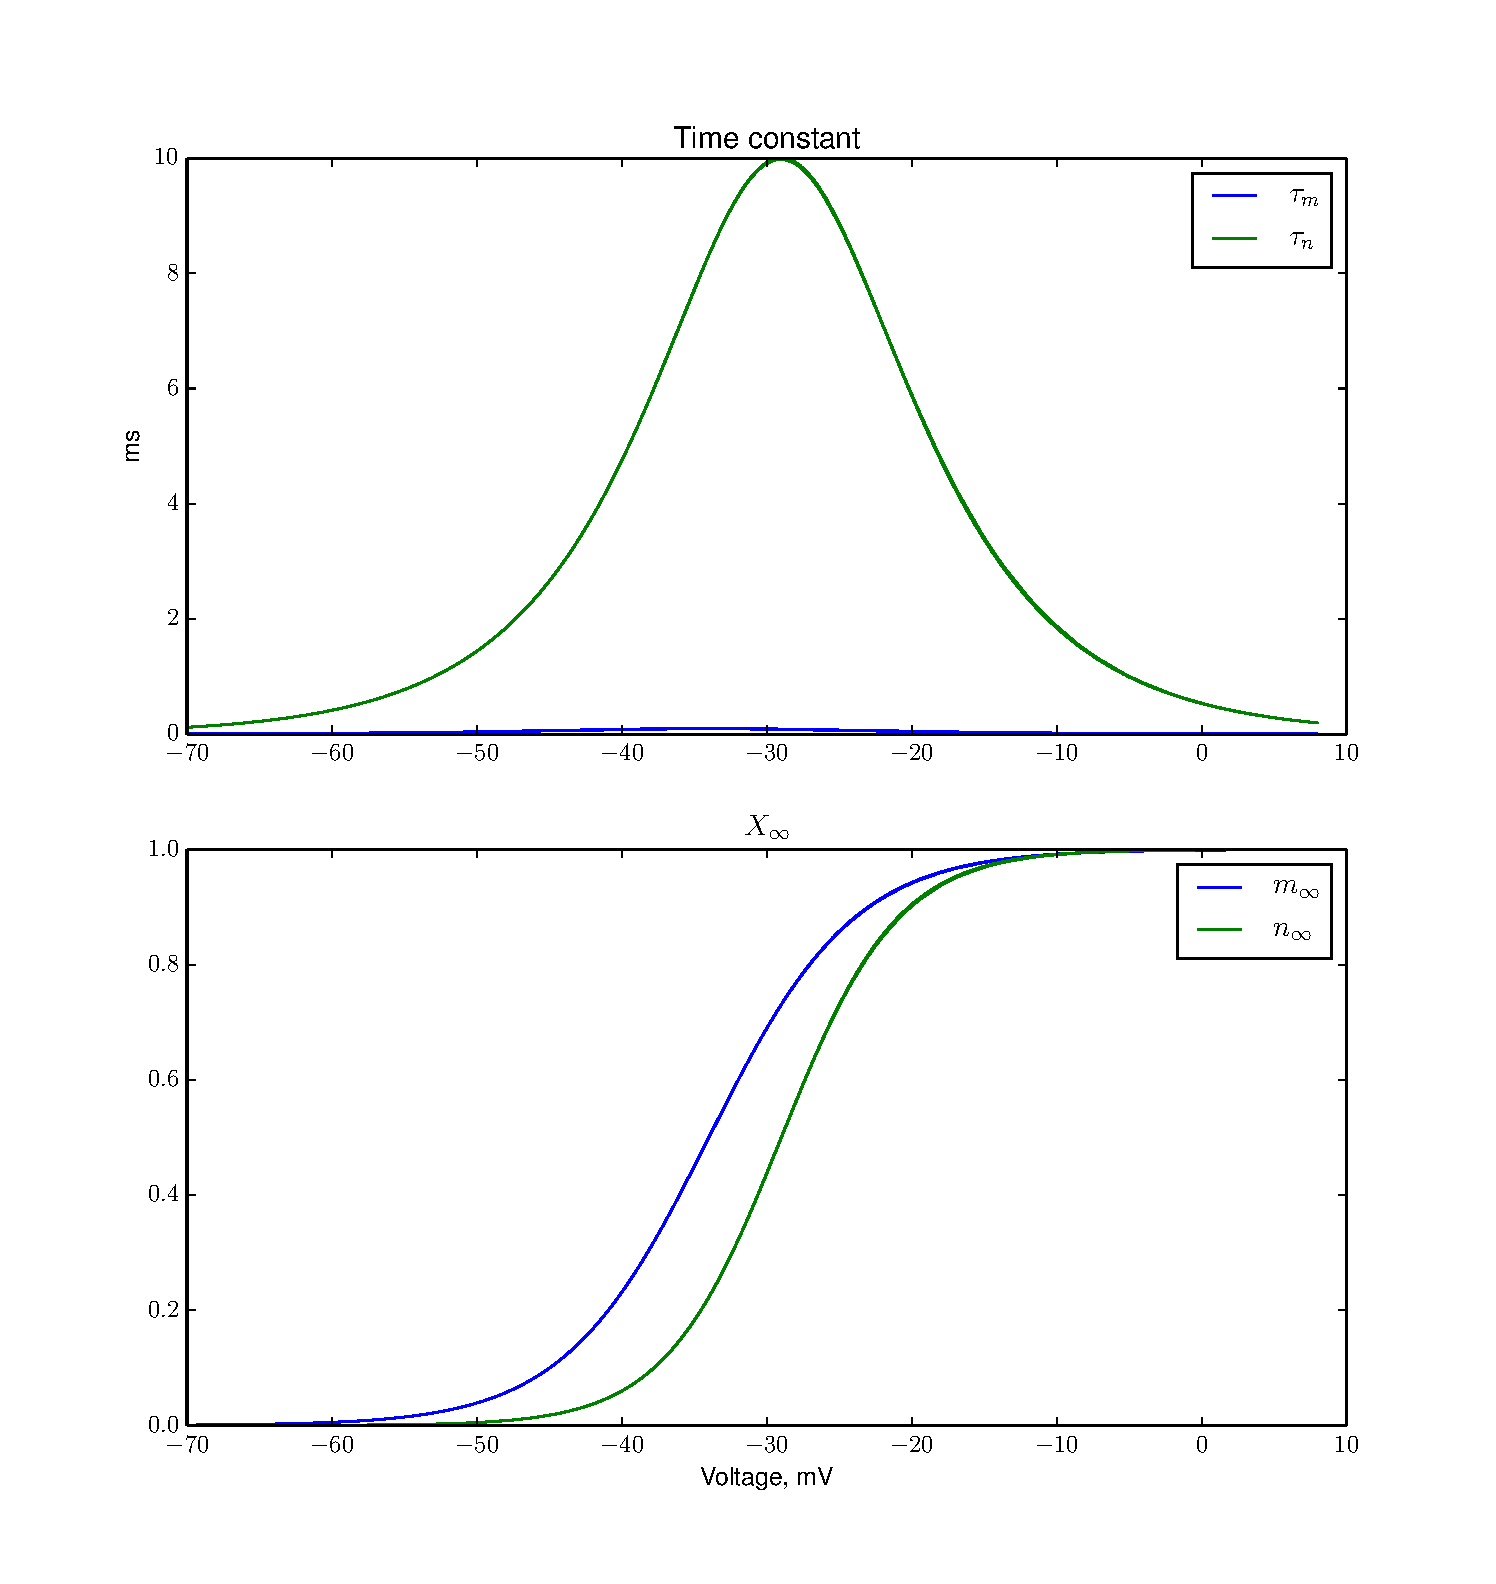
\includegraphics[width=\textwidth]{tau_inf}
    \caption{Effect of time parameters on m and n}
    \label{fig:tau_inf}
\end{figure}

\section{Bursting neuron}

In this exercise, we add two persistent channels, one for sodium
and one for potassium.

\subsection{Persistent sodium channel for repetitive firing}

Our approach for finding a threshold for sustained repetitive
firing is refinement based : we start by testing if the neuron
shows sustained repetitive firing for several ascending values.
Once we hit a value for $\tilde{g}_{NaP}$ for the neuron having
such a behaviour, we start at that value minus the chosen step,
but this time with a smaller step. We repeat this until the
precision seems good enough.

To test if the neuron shows sustained firing, we simply count
the number of spikes for the whole simulation, and if this number
is small (less than 10 in our case), we assume that the neuron is
not undergoing sustained repetitive firing.

We found the threshold value for $\tilde{g}_{NaP}$ when it can evoke bursting 
with the precision of 0.1 nS. It turned out to be 2.35.

The figure \ref{fig:2.1} shows appearance of the bursting behavior evoked by 
persistent sodium channel $NaP$. The conductance $\tilde{g}_{NaP}$ was
set to $3.0 nS$ to visualize the typical case. Neuron does not return
to rest because the channel $NaP$ stays open longer than the usual $Na$ channel
while the voltage falls down. This sustained current evokes action potential
again. The reason of that is that conductance of normal $Na$ channel is 
proportional to cube of gating variable $m$ whereas there is a linear dependence
between conductance and gating variable $r$ for channel $NaP$.

\begin{figure}[H]
    \centering
    \includegraphics[width=\textwidth]{ex2_1}
    \caption{Result of simulation with the persistent sodium channel NaP}
    \label{fig:2.1}
\end{figure}

\subsection{Slow potassium channel for bursting}

Further modification of the neuron model introduces slow potassium channel $KS$
which ends bursting behavior. The figures \ref{fig:short} and \ref{fig:long}
demonstrates the simulations with channel $KS$ for short (20 ms) and long ($10^4$ms) injected
current pulse of 40pA respectively.

With the short pulse we can observe long bursting period
which strongly exceeds the pulse duration. Since the voltage stays high during bursting
conductance of $KS$ channel slowly grows until it becomes high enough to end firing.
The dynamics of $KS$ conductance is much slower than of the others because of the parameter $\bar{\tau}_k$.

\begin{figure}[H]
    \centering
    \includegraphics[width=\textwidth]{ex2_2_short}
    \caption{Result of simulation with the persistent potassium channel KS (short pulse)}
    \label{fig:short}
\end{figure}

Long pulse uncovers transient behavior in the beginning though eventually the neuron
switches to the bursting. We can see how the conductance of $KS$ changes via looking
at the dynamics of pick currents (during spikes). When it is low, the bursting start
is caused by the gradual growth of voltage via $NaP$ channel. When the $KS$ conductance
reaches particular value the bursting end.

\begin{figure}[H]
    \centering
    \includegraphics[width=\textwidth]{ex2_2_long}
    \caption{Result of simulation with the persistent potassium channel KS (long pulse)}
    \label{fig:long}
\end{figure}

\section{Analysis of bursting and beating behaviors}
\subsection{Description of repetitive bursting}

To measure the repetitive bursting behavior observed in the previous exercise
we implemented a function estimating duration of each burst and the period of
burst repetition. We used a couple of arbitrary but reasonable for this task thresholds.
First of all we detect all spikes using the previously used function. Then we 
extract the times of the first spikes in bursting set.
Bursting set is supposed to be finished if there is no spike during 200 ms after the last one.
To deal with the transient behavior in the beginning we cut out all found ``bursting'' sets of size
less than 10 spikes in the beginning. Then the period of the burst is the difference in times
between the first spikes of neighboring bursts. Duration is the difference in times between the
first spike of the set and the spike preceding the first spike of the following set.
If there is only one burst we set the period to 10$s$.

For the simulations in this section we used $\tilde{g}_{NaP} = 3.2nS$, pulse
duration of 10$s$ and varied injected current from 5 to 45 pA.
We can see how the period and duration of bursting sets changes with 
the current on the figure \ref{fig:bdur_bper}.

From the figure We can conclude that the duration does not depend much on the
injected current while the period becomes shorter.

\begin{figure}[H]
    \centering
    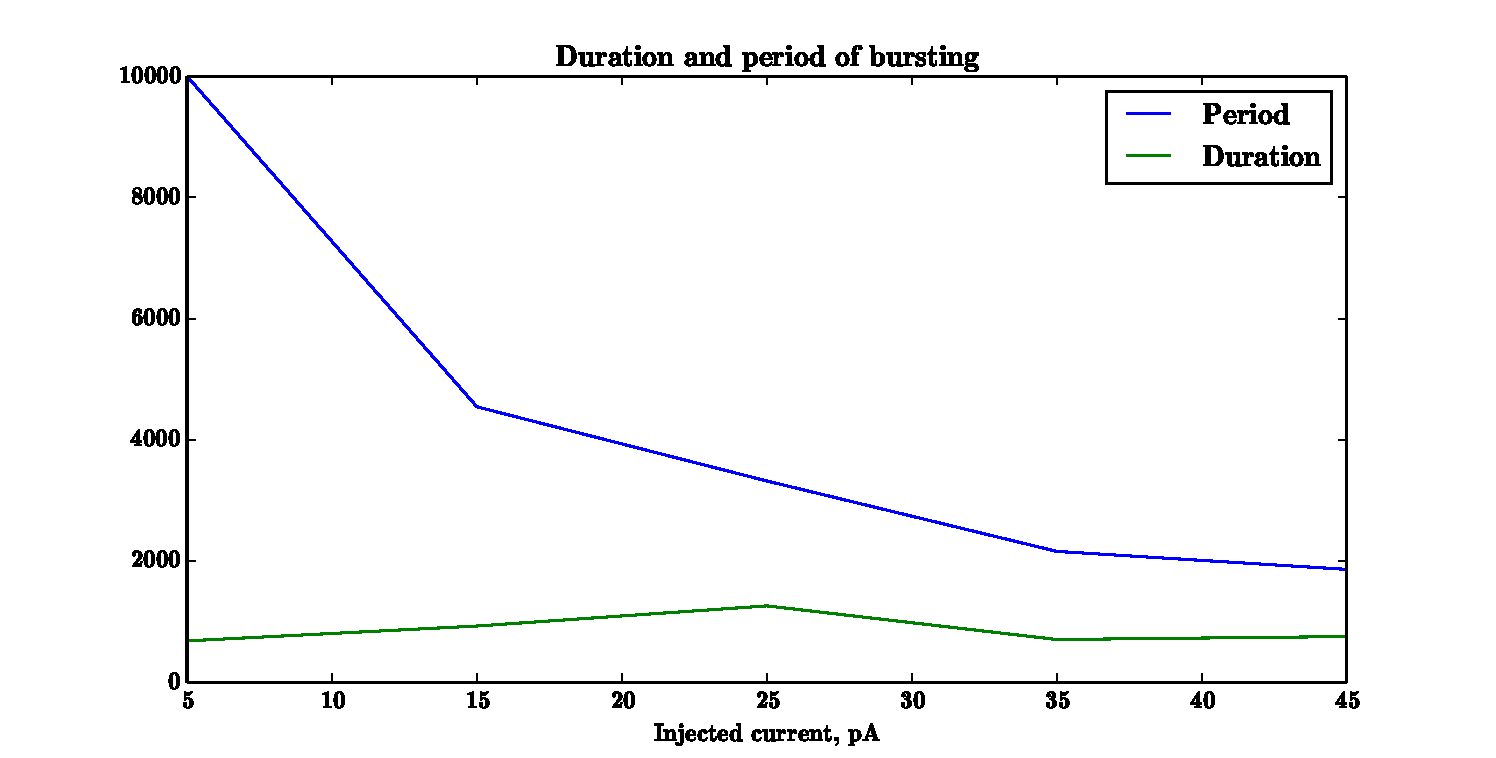
\includegraphics[width=0.7\textwidth]{bduration_bperiod}
    \caption{Duration and period of the bursting for different injected currents}
    \label{fig:bdur_bper}
\end{figure}

\subsection{Bursting and beating modes}

This section is dedicated to beating behavior which
can be observed for high injected current. The figure \ref{fig:beat} was obtained
with $\tilde{g}_{NaP} = 3.2nS, I_{ext} = 80pA$, and the pulse duration of 10$s$.
This new beating behavior occurs probably because the external current is so
large that $KS$ channel cannot block the positive current even with
its maximal possible conductance. 

\begin{figure}[H]
    \centering
    \includegraphics[width=\textwidth]{ex3_2}
    \caption{Simulation for beating mode}
    \label{fig:beat}
\end{figure}


\subsection{Phase diagram}

In this section we analyze different modes of neuronal behavior
depending on the parameters  $\tilde{g}_{NaP} and I_{ext}$.
In order to classify the mode we modified the function of the Exercise 3.1.
After removal of transients in the beginning we classify as silence in
the absence of bursts and as beating if the duration of a ``burst'' is more than 1.5$s$.
The interval between spikes for bursting is computed as average of all the intervals.

The results can be found on the figure \ref{fig:modes}. In case of bursting
the frequency is the frequency of bursting sets (which is inverse of the period),
for the beating it is the frequency of spikes. We explored the following intervals of
parameters: $0 < I_{ext} < 80pA and 1.5nS < \tilde{g}_{NaP} < 3.5nS$, with
the stimulus duration of 12$s$.

The mode depends on both injected current and $NaP$ channel conductance.
Starting from at least 70pA the neuron elicits beating no matter what the conductance is
in the defined interval. The transition from silence to bursting occurs after 10pA
for conductances lower than 2.5 and even earlier for the larger conductances.

\begin{figure}[H]
    \centering
    \includegraphics[width=\textwidth]{ex3_3}
    \caption{Modes and frequencies for different injected current and conductances $\tilde{g}_{NaP}$}
    \label{fig:modes}
\end{figure}

\end{document}
